\section{Falsifiability and fingerprints}\label{sec:falsifiability}

The review is conceptual, but not meant to be unfalsifiable. The superspace/readout framework suggests concrete statistical signatures that can be tested in numerical experiments and, in some cases, in laboratory analogues (e.g.\ optical interference patterns or engineered quasi-periodic media). We list a minimal set of fingerprints that are both natural and robust under moderate protocol variations.

\subsection{Candidate laboratory platforms (where the pipeline can be tested)}\label{sec:falsifiability:platforms}

While our primary demonstrations are numerical, the same ``geometry $\to$ readout $\to$ stabilization $\to$ time'' pipeline matches the data products available in several laboratory platforms:
\begin{itemize}[leftmargin=*,itemsep=2pt]
  \item \textbf{Photonic quasicrystals / aperiodic photonic lattices}: far-field diffraction and structure-factor measurements directly probe module-supported peak locations and window-envelope effects (Section~\ref{sec:falsifiability:diffraction}). Resolution parameters $\epsilon$ map to finite numerical aperture, bandwidth, detector point spread, or deliberate kernel smoothing in reconstruction pipelines.\cite{Lahini2009}
  \item \textbf{Cold atoms in quasiperiodic optical lattices (Aubry--Andr{\'e}/Harper; Fibonacci modulations)}: time series of density/occupation and momentum-space images provide both spectral fingerprints and long symbolic records after thresholding or multi-level binning. Here $\epsilon$ can be operationalized as controlled disorder strength, imaging resolution, or deliberate coarse-graining of the measurement record.\cite{Roati2008}
  \item \textbf{Driven spin chains / superconducting-qubit arrays with quasiperiodic modulation}: continuous or repeated projective readout produces long, protocol-defined records with realistic temporally correlated noise, making the correlated-noise skew-product formulation (Section~\ref{sec:readout:probabilistic-template}) directly testable. Stabilization/folding then becomes a transparent post-processing layer whose robustness can be quantified by mismatch and finite-sample error bars.\cite{SpethmannStanoLoss2025SpinQubitHMM}
\end{itemize}

In all cases, the conservative falsifiable content is protocol-level: one specifies the measurement channel $\Theta$ (including resolution, filtering, and stabilization), reports finite-size uncertainty budgets, and tests whether the predicted invariants (peak locations/envelopes, visibility curves, stabilized degeneracy statistics, and entropy/time growth classes) are reproducible across phases and robust under admissible protocol perturbations.

\subsection{Quasiperiodic diffraction and spectral fingerprints}\label{sec:falsifiability:diffraction}

Regular model sets have pure-point diffraction under broad conditions, with Bragg peaks located on a Fourier module determined by the underlying lattice and the star map \cite{Hof1995,BaakeGrimm2013}. In the present context, this suggests:
\begin{itemize}[leftmargin=*,itemsep=2pt]
  \item the \emph{geometric primitive} (CPS) constrains the locations of spectral lines;
  \item the \emph{window} and its boundary regularity control peak intensities and continuous components.
\end{itemize}
Protocol-level falsification: given a proposed CPS and window family, simulate $\Lambda(W)$ on increasing finite patches and compute empirical diffraction; check convergence to the predicted module and intensity envelope.

\subsubsection{A standard intensity formula and the role of resolution}\label{sec:falsifiability:diffraction-formula}

For regular (and more generally weighted) model sets, there is a precise link between window geometry in internal space and observed Bragg peak intensities. A convenient summary (see e.g.\ \cite{Hof1995,BaakeGrimm2013}) is that, for wave vectors $k$ in the Fourier module determined by the CPS, the Bragg peak intensity takes the form
\[
I(k)\ \propto\ \bigl|\widehat{w}(k^\star)\bigr|^2,
\]
where $w:H\to\RR$ is the window weight (sharp: $w=\mathds{1}_W$; fuzzy/finite resolution: $w=\kappa_\epsilon$), $k^\star$ denotes the internal-space counterpart of $k$ under the star map on the dual module, and $\widehat{w}$ is the Fourier transform on $H$.

\begin{remark}[A concrete Fourier convention]\label{rem:fourier-convention}
To avoid convention ambiguity when discussing ``Fourier coefficients of the window'', one may fix the convention
\[
\widehat{w}(\xi):=\int_H w(y)\,e^{-2\pi i \langle \xi,y\rangle}\,\mathrm{d}y,\qquad \xi\in H^\ast,
\]
with $\mathrm{d}y$ the Lebesgue/Haar measure on $H$. With this choice, closed-form window transforms (e.g.\ boxes) can be written explicitly and compared directly to intensity envelopes.
\end{remark}

\begin{proposition}[Pure-point diffraction and an intensity formula]\label{prop:diffraction-intensity}
For a regular model set arising from a cut-and-project scheme (with $\partial W$ of Haar measure zero) and for bounded Riemann-integrable window weights $w$ (including $w=\mathds{1}_W$ and smooth kernels $\kappa_\epsilon$), the diffraction measure is pure point and supported on a Fourier module determined by the dual lattice and the star map. For $k$ in this module, the corresponding Bragg intensity is proportional to $|\widehat w(k^\star)|^2$ (up to a CPS-dependent density/normalization factor).
\cite{Hof1995,BaakeGrimm2013,RichardStrungaru2017}
\end{proposition}

\paragraph{Closed-form example: a box window.}
If $H=\RR^n$ and one chooses a (polytope) window weight given by an axis-aligned box
\[
w(y)=\mathds{1}_{\prod_{j=1}^n[-L_j/2,L_j/2]}(y),
\]
then under the convention of Remark~\ref{rem:fourier-convention} one has the explicit product formula
\[
\widehat w(\xi)=\prod_{j=1}^n \left(L_j\,\mathrm{sinc}(L_j \xi_j)\right),
\qquad
\mathrm{sinc}(z):=\frac{\sin(\pi z)}{\pi z},
\]
with the standard continuous extension $\mathrm{sinc}(0)=1$. This is a simple instance of the broader LCA-group/Poisson-summation framework for model-set diffraction and is particularly convenient for protocol auditability: it provides a closed-form intensity envelope against which finite-patch diffraction estimates can be compared.

\paragraph{Estimating window Fourier coefficients from finite readout.}
Given a finite patch $\{x_i\}_{i=1}^N\subset E$ from a proposed model set and a set of candidate module wave vectors $k$, one can estimate a structure factor
\[
\widehat\rho_N(k):=\frac{1}{N}\sum_{i=1}^N e^{-2\pi i\langle k,x_i\rangle},
\qquad
S_N(k):=|\widehat\rho_N(k)|^2.
\]
Phase averaging over internal shifts $u$ (or over scan phases in the protocol) reduces fluctuations and isolates the module-supported peaks. In a geometry-first test where the Fourier module and the star map are specified by the CPS, one then regresses the phase-averaged peak intensities against the predicted window envelope $|\widehat w(k^\star)|^2$ (or fits window parameters $L_j$ in the box case). The key falsifiable content is not the exact normalization constant, but the \emph{relative} intensity profile across module points as a function of $k^\star$ and the controlled dependence on the resolution parameter $\epsilon$ through the choice $w=\kappa_\epsilon$.

\begin{remark}[From readout to $\widehat w$: a minimal estimation workflow]\label{rem:estimate-window-fourier}
To connect data directly to the window Fourier coefficients in Proposition~\ref{prop:diffraction-intensity}, the minimal auditable workflow is:
\begin{enumerate}[label=(\roman*),leftmargin=*,itemsep=2pt]
  \item specify the CPS (hence the Fourier module and the star map $k\mapsto k^\star$);
  \item select a finite set of candidate module vectors $\{k\}$ (e.g.\ by dual-lattice enumeration with a cutoff);
  \item estimate $S_N(k)$ from the observed point patch (and phase-average over internal shifts/phases);
  \item remove the unknown global normalization by working with ratios or by normalizing by $\max_k S_N(k)$ on the chosen set;
  \item fit the window parameters by matching $S_N(k)$ to $|\widehat w(k^\star)|^2$ (closed form for boxes; numerical quadrature/FFT for more general polytopes).
\end{enumerate}
The demo scripts implement this workflow explicitly for a box window (closed-form $\widehat w$) and compare the normalized envelope to normalized empirical intensities.\cite{RichardStrungaru2017}
\end{remark}

This identity explains two protocol-facing facts:
\begin{itemize}[leftmargin=*,itemsep=2pt]
  \item \textbf{Window geometry controls intensities}: changing $W$ (or using a weight $w$) changes $\widehat w$ and hence the intensity envelope without moving the Fourier module itself.
  \item \textbf{Resolution acts as spectral smoothing}: replacing a sharp indicator by a smoothed kernel $\kappa_\epsilon$ suppresses high-frequency features of $\widehat w$. In practice, increasing $\epsilon$ corresponds to stronger attenuation of fine-scale internal-space boundary structure, and therefore to weaker contrast in the high-$|k^\star|$ regime.
\end{itemize}

The numerical FFT-based fingerprints in Demos B--C are finite-patch, finite-grid approximations of this principle. In those scripts, the visibility curve $V(\epsilon)$ is a compressed contrast statistic derived from the binned intensity/density (variance over mean). While $V(\epsilon)$ is not itself a Bragg intensity, it is sensitive to the same mechanism: as $\epsilon$ increases, the effective weight $w=\kappa_\epsilon$ becomes smoother, which reduces the prominence of sharp interference features and typically lowers contrast at fixed discretization, up to quasi-periodic modulation tied to the Fourier module and to phase averaging.

\begin{proposition}[P1: quasiperiodic spectral lines as a model-set signature]\label{prop:P1}
If a visible 3D point set arises (to the accuracy of the protocol) from a regular cut-and-project model set, then its diffraction/structure factor is expected to be dominated by discrete Bragg peaks supported on a Fourier module determined by the superspace lattice and the star map. Variations of internal phase $u$ should produce structured phase shifts rather than uncorrelated drifts.
\end{proposition}

\subsection{Resolution-dependent visibility curves}\label{sec:falsifiability:visibility}

Finite-resolution readout replaces sharp acceptance by kernels. This suggests a generic family of \emph{visibility curves}: as resolution increases (kernel narrows), interference-like contrast measures should change in predictable ways because more boundary structure becomes resolvable. One can operationalize this without committing to a specific physical interferometer:
\begin{itemize}[leftmargin=*,itemsep=2pt]
  \item choose a resolution parameter $\epsilon$ controlling window fuzzification;
  \item define a contrast statistic $V(\epsilon)$ based on the variance of readout intensities or on autocorrelation of symbolic sequences;
  \item test whether $V(\epsilon)$ follows the scaling predicted by the window boundary geometry (e.g.\ via Minkowski content heuristics) and by the induced symbolic complexity.
\end{itemize}
While the precise scaling depends on the protocol, the key falsifiable content is \emph{monotone and scale-structured} dependence on $\epsilon$ with quasi-periodic modulation tied to the superspace module.

\begin{proposition}[P2: golden-branch slopes and Diophantine minimal-resonance]\label{prop:P2}
Consider a one-dimensional torus scan $x_t=x_0+t\alpha\ (\mathrm{mod}\ 1)$ with slope $\alpha\in(0,1)\setminus\QQ$.
Write $\|y\|:=\min_{p\in\ZZ}|y-p|$ for distance to the nearest integer, and define the \emph{asymptotic resonance constant}
\[
c(\alpha):=\liminf_{q\to\infty} q\,\|q\alpha\|.
\]
Then one has the sharp universal bound
\[
c(\alpha)\ \le\ \frac{1}{\sqrt5}\qquad\text{for every irrational }\alpha,
\]
and the constant $1/\sqrt5$ is optimal in the sense that it is attained (as a liminf along an explicit subsequence) by the golden ratio slope $\alpha=\varphi-1$, where $\varphi=(1+\sqrt5)/2$.
Moreover, if $c(\alpha)=1/\sqrt5$, then $\alpha$ lies in the modular (fractional-linear) equivalence class of $\varphi-1$ (Markov/Lagrange spectrum rigidity).
\end{proposition}

\begin{proof}
The inequality $c(\alpha)\le 1/\sqrt5$ is a direct reformulation of Hurwitz's theorem: for every irrational $\alpha$ there exist infinitely many rationals $p/q$ with
\[
\left|\alpha-\frac{p}{q}\right|<\frac{1}{\sqrt5\,q^2}.
\]
For such $p/q$ one has $\|q\alpha\|=|q\alpha-p|=q\left|\alpha-\tfrac{p}{q}\right|<\tfrac{1}{\sqrt5\,q}$, hence $q\|q\alpha\|<1/\sqrt5$ along infinitely many $q$, which implies $c(\alpha)\le 1/\sqrt5$.
\cite{Cassels1957DiophantineApproximation,Khinchin1964ContinuedFractions}

For sharpness, take $\alpha=\varphi-1$ whose continued fraction is $[0;1,1,1,\dots]$.
Let $p_n/q_n$ be its convergents; then $(q_n)$ are Fibonacci numbers up to an index shift.
Let $\alpha_{n+1}:=[1;1,1,\dots]=\varphi$ denote the (constant) tail of the continued fraction after the $n$-th digit.
The standard continued-fraction recombination identity gives
\[
\alpha=\frac{p_n\alpha_{n+1}+p_{n-1}}{q_n\alpha_{n+1}+q_{n-1}}.
\]
Using the determinant relation $p_n q_{n-1}-p_{n-1}q_n = (-1)^{n-1}$, one computes
\[
\left|\alpha-\frac{p_n}{q_n}\right|
=\frac{1}{q_n\,(q_n\alpha_{n+1}+q_{n-1})},
\qquad\text{hence}\qquad
q_n\|q_n\alpha\|
=q_n^2\left|\alpha-\tfrac{p_n}{q_n}\right|
=\frac{1}{\alpha_{n+1}+q_{n-1}/q_n}.
\]
Since $\alpha_{n+1}=\varphi$ and $q_{n-1}/q_n\to \varphi^{-1}$ for Fibonacci denominators, we obtain
\[
\lim_{n\to\infty} q_n\|q_n\alpha\|
=\frac{1}{\varphi+\varphi^{-1}}
=\frac{1}{\sqrt5},
\]
and therefore $c(\varphi-1)=1/\sqrt5$.
\cite{Khinchin1964ContinuedFractions}

Finally, the rigidity statement that equality $c(\alpha)=1/\sqrt5$ characterizes the modular equivalence class of $\varphi-1$ is a classical theorem in the theory of the Markov/Lagrange spectra.\cite{CusickFlahive1989MarkovLagrangeSpectra}
\end{proof}

\begin{remark}[Finite resources and protocol-facing interpretation]
For a finite scan depth $Q$, a conservative ``locking'' proxy is $\min_{1\le q\le Q}\|q\alpha\|$: small values correspond to near-periodic recurrences at scale $q$.
Proposition~\ref{prop:P2} shows that the golden-ratio slope (and its modular equivalents) maximizes the asymptotic obstruction to such resonances in the sharp Hurwitz sense.
Connecting this to finite-$Q$ discrepancy and gap-statistic optimality requires specifying the exact observable (e.g.\ discrepancy of $\{t\alpha\}$, or three-gap counts for the induced cylinder partition); the proof above isolates the minimal-input, fully rigorous core of the ``minimal resonance'' claim.
\end{remark}

\subsection{Folding/degeneracy counts as discrete invariants}\label{sec:falsifiability:folding}

Stabilization maps $\Fold_m$ induce a finite partition of raw readout words into stable types (Section~\ref{sec:stabilization}). Two robust invariants are:
\begin{enumerate}[label=(\roman*),leftmargin=*,itemsep=2pt]
  \item the \emph{type count} $|X_m|$ (often Fibonacci for golden-mean constraints);
  \item the \emph{degeneracy spectrum} $\{|\mathcal{F}_m(x)|: x\in X_m\}$.
\end{enumerate}
Protocol-level falsification: compute empirical frequencies of stabilized types and compare to the predicted maximum-entropy (or invariant-measure-induced) distribution; compare degeneracy counts across resolutions $m$ and check for renormalization relations (e.g.\ Fibonacci scaling under substitution).

\begin{proposition}[P3: degeneracy histograms as reproducible combinatorial invariants]\label{prop:P3}
Fix a stabilization rule $\Fold_m$ and a word length $m$. The multiset of fiber sizes $\{|\mathcal{F}_m(x)|:x\in X_m\}$ (the ``degeneracy histogram'') is a discrete, reproducible combinatorial invariant of the protocol. Platforms that share the same stabilization grammar and decoding rule should exhibit the same histogram when their raw records are recoded into stabilized types.
\end{proposition}

\subsection{Delayed-choice phenomena as protocol refactorization}\label{sec:falsifiability:delayed-choice}

In many ``delayed-choice'' experimental narratives, changing the measurement setting after a signal has propagated appears to retroactively change the ``past'' behavior. In the readout-based framework, a conservative protocol-level explanation is available: the underlying object-level structure is static (or at least fixed during the run), while the measurement change modifies the \emph{readout operator} and hence the equivalence-class decomposition of the same underlying microstates.

\begin{proposition}[P4: equivalence-class reallocation test]\label{prop:P4}
Assume a delayed change of measurement corresponds to changing readout parameters (window/kernel/projection) and hence changing the induced stabilization map on recorded data. Then the observed statistical changes should be explainable by a computable reallocation of weights between stabilized types, subject to conservation constraints determined by the stabilization grammar (e.g.\ total weight conservation and reachability constraints on type-to-type transfers).
\end{proposition}

\subsection{Closed-loop adaptive observers and stability transitions}\label{sec:falsifiability:adaptive}

A distinctive feature of protocol-based reconstruction is that the observer may be modeled as an adaptive system: parameters $\Theta$ are updated based on accumulated readout data. This makes it possible to formulate falsifiable convergence/phase-transition claims for the protocol itself, independent of any ontological randomness.

\begin{proposition}[P5: observable convergence domains in adaptive protocols]\label{prop:P5}
Suppose the observer updates its protocol parameters by approximately descending a mismatch functional (a loss defined on readout statistics). Then one expects the existence of empirically detectable convergence domains and transition boundaries: beyond a threshold of disturbance or resource constraints, the protocol exits a stable-type regime and enters a defect-accumulation regime, with measurable growth of mismatch and collapse of stabilized-type persistence.
\end{proposition}

\subsection{Minimal reproducible numerical protocol}\label{sec:falsifiability:protocol}

To make the above fingerprints auditable, a minimal reproducible workflow is:
\begin{enumerate}[label=\textbf{P\arabic*.},leftmargin=*,itemsep=2pt]
  \item Specify CPS data $(E,H,\Gamma)$ and window family $W_\epsilon$ (including parameterization and boundary regularity assumptions).
  \item Fix scan dynamics on internal space (e.g.\ $h_t=h_0+t\alpha$) and a readout map $R_\Theta$ (binary or multi-symbol).
  \item Generate (i) finite patches of $\Lambda(W_\epsilon)$, and (ii) symbolic sequences of length $T$ for multiple phases $h_0$.
  \item Compute: diffraction estimates, visibility statistics $V(\epsilon)$, symbolic complexity/entropy estimates, and stabilization counts for $\Fold_m$.
  \item Compare to predicted invariants (Fourier module, scaling laws, Fibonacci counts, entropy rates) with error bars from finite-size effects.
\end{enumerate}

This protocol is intentionally agnostic about the physical interpretation; it is designed to test whether the \emph{geometric+protocol} chain yields stable, reproducible signatures.

\subsection{Minimal numerical demonstration (this paper)}\label{sec:falsifiability:demo}

To address the auditability gap between ``fingerprints'' and concrete realizations, this repository includes three minimal demonstrations generated by a single command:
\[
\texttt{python3 scripts/run\_all.py}.
\]
The outputs are written under \texttt{artifacts/} together with a parameter file and a run log.
\begin{itemize}[leftmargin=*,itemsep=2pt]
  \item \textbf{Demo A (1D, zero KS entropy)}: an irrational rotation with a two-interval readout (Sturmian regime). We compute exact cylinder measures and visualize the sublinear growth of $\tau(t)$ (Figures~\ref{fig:demo1d-tau}--\ref{fig:demo1d-entropy}), clarifying how the protocol refinement functional behaves at $h_\mu(T)=0$.
  \item \textbf{Demo B (2D $\rightarrow$ 1D Fibonacci model set)}: a cut-and-project construction from $\ZZ^2$ with a compact window. We show a finite-patch structure factor and a resolution-dependent visibility curve $V(\epsilon)$ with phase averaging, as well as an exact (combinatorial) degeneracy histogram for a simple Zeckendorf-based $\Fold_m$.
  \item \textbf{Demo C (6D $\rightarrow$ 3D icosahedral approximation)}: a $\ZZ^6$ cut-and-project construction with a golden-ratio-based icosahedral splitting and a compact internal-space window (spherical, boundary measure zero). We show a diffraction slice and a phase-averaged visibility curve $V(\epsilon)$ under window fuzzification, and we additionally run an internal-phase scan with a probabilistic window kernel to produce a symbolic record whose entropy-rate proxy varies with $\epsilon$ (Figure~\ref{fig:demo6d-entropy-rate}). The same record is stabilized by a Zeckendorf $\Fold_m$ to produce reproducible fiber/transition statistics stored in \texttt{artifacts/demo\_6d\_fingerprints.json}.
\end{itemize}

\begin{remark}[Numerical tests of the listed fingerprints]\label{rem:fingerprint-tests}
In addition to producing plots, the repository includes a small set of scalar pass/fail checks that operationalize parts of Propositions~\ref{prop:P1}--\ref{prop:P3} on the generated data. Running
\[
\texttt{python3 scripts/run\_all.py}
\]
also produces \texttt{artifacts/fingerprint\_tests.json}, which records (i) a zero-entropy sanity check for Demo~A via block-entropy growth, (ii) exact Fold degeneracy invariants $\sum_x|\mathcal{F}_m(x)|=|\mathcal{A}|^m$ and $|X_m|=F_{m+2}$ (Proposition~\ref{prop:fiber-partition}) for the chosen $m$, and (iii) a quantitative goodness-of-fit statistic comparing an empirical structure factor against the closed-form box-window envelope $|\widehat w(k^\star)|^2$ in Demo~C (Proposition~\ref{prop:diffraction-intensity}).
\end{remark}

\begin{table}[t]
  \centering
  \caption{End-to-end numerical demonstration: where each fingerprint is instantiated and how to audit it. All files are generated by \texttt{python3 scripts/run\_all.py}; JSON artifacts are written under \texttt{artifacts/} and figures/snippets under \texttt{sections/generated/}.}
  \label{tab:fingerprint-audit-map}
  \begin{tabular}{@{}p{0.22\linewidth}p{0.36\linewidth}p{0.34\linewidth}@{}}
    \toprule
    Fingerprint (paper) & What is computed (demo output) & Where to audit (file / figure) \\
    \midrule
    Diffraction module/envelope (P1) &
    Empirical structure factor vs.\ closed-form window envelope (box window variant) &
    \texttt{artifacts/demo\_6d\_box\_window\_fourier.json};
    \texttt{sections/generated/demo\_6d\_box\_window\_envelope\_scatter.png} \\
    \addlinespace
    Visibility transition under fuzzification (P2) &
    Phase-averaged visibility curve \(V(\epsilon)\) &
    Figure~\ref{fig:demo6d-visibility} (\texttt{sections/generated/demo\_6d\_visibility\_curve.png});
    \texttt{artifacts/demo\_6d\_fingerprints.json} \\
    \addlinespace
    Entropy-rate time under probabilistic readout (protocol time) &
    \(\epsilon\mapsto \widehat h(\epsilon)\) and a \(\widehat\tau(t)\) proxy &
    Figure~\ref{fig:demo6d-entropy-rate} (\texttt{sections/generated/demo\_6d\_entropy\_rate\_proxy.png});
    \texttt{sections/generated/demo\_6d\_tau\_markov.png};
    \texttt{artifacts/demo\_6d\_fingerprints.json} \\
    \addlinespace
    Fold/fiber degeneracy statistics (P3) &
    Exact degeneracy histogram, type frequencies, transition counts, exact Fold transition graph &
    \texttt{artifacts/demo\_6d\_fingerprints.json};
    \texttt{artifacts/demo\_6d\_fold\_graph\_m12.json};
    \texttt{sections/generated/demo\_6d\_fold\_graph\_m12\_heatmap.png};
    \texttt{artifacts/fingerprint\_tests.json} \\
    \addlinespace
    Ring-factor / rational-approximant diagnostics (protocol control) &
    Three-gap statistics, convergent checks, mismatch diagnostics; Sturmian block complexity and fuzzy-readout entropy &
    \texttt{sections/generated/demo\_6d\_1d\_factor\_gap\_stats.png};
    \texttt{sections/generated/demo\_6d\_ring\_factor\_complexity.png};
    \texttt{sections/generated/demo\_6d\_ring\_entropy\_rate\_proxy.png};
    \texttt{artifacts/demo\_6d\_fingerprints.json} \\
    \bottomrule
  \end{tabular}
\end{table}

\begin{remark}[Protocol-equivalence invariance: what is robust, what is not]\label{rem:fingerprint-protocol-invariance}
The listed fingerprints mix object-layer constraints (geometry/spectrum) with protocol-layer choices (readout, stabilization, factor selection).
To avoid over-claiming, it is useful to fix an \emph{acceptable protocol class} and state invariance only within that class.
A conservative choice is:
\begin{itemize}[leftmargin=*,itemsep=2pt]
  \item \textbf{MEF-adapted readouts}: protocols whose deterministic component factors through the maximal equicontinuous factor (Definition~\ref{def:mef-adapted-protocol}), so that different choices of ring-factor $\phi$ are compared on the same canonical base (Remark~\ref{rem:phi-same-mef}).
  \item \textbf{Finite-memory recodings}: protocols related by sliding-block (finite-memory) equivalence of their symbol streams (Definition~\ref{def:finite-memory-equivalence}), so that growth laws of $\tau(t)$ are stable up to $O(1)$ alignment (Corollary~\ref{cor:tau-affine-class}).
  \item \textbf{Small window/partition perturbations}: protocols whose one-step mismatch is small (Definition~\ref{def:mismatch-rate}), so that induced changes in block laws and entropy rates are quantitatively controlled (Propositions~\ref{prop:block-tv-by-mismatch} and \ref{prop:entropy-continuity-mismatch}).
\end{itemize}
Within such a class, the strongest invariances are those determined by the object layer or by discrete stabilization grammar:
\begin{itemize}[leftmargin=*,itemsep=2pt]
  \item \textbf{Geometric/spectral constraints} (e.g.\ Fourier module locations, envelope classes) are fixed by the superspace CPS and window family.
  \item \textbf{Fold/fiber degeneracy invariants} at fixed $m$ are discrete combinatorial properties of the stabilization rule (Proposition~\ref{prop:P3}) and persist across equivalent recodings that do not change the stabilization grammar.
\end{itemize}
By contrast, protocol curves such as $\epsilon\mapsto \widehat h(\epsilon)$, numerical discrepancy values, and specific gap statistics are \emph{not} claimed to be strictly invariant under changing $\phi$ or window/partition choice; their intended falsifiable content is stability \emph{as a class} (e.g.\ growth class, monotone trends, and quantitative error bars under mismatch), rather than equality of point estimates across all protocols.
\end{remark}

\begin{figure}[t]
  \centering
  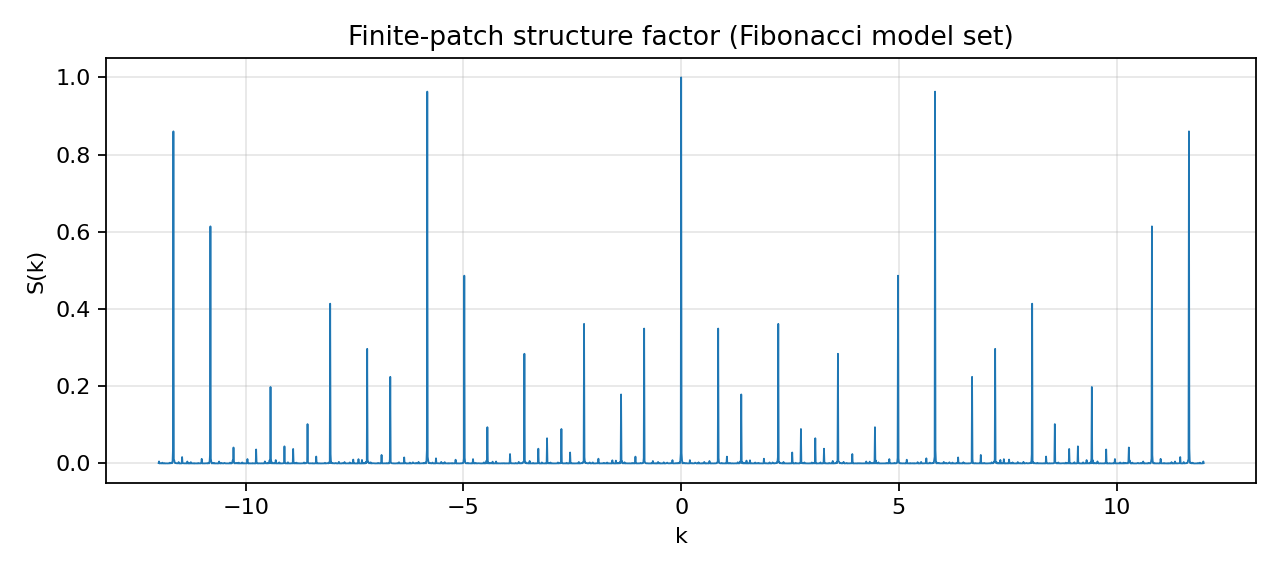
\includegraphics[width=0.95\linewidth]{sections/generated/demo_2d_diffraction.png}
  \caption{Demo B: finite-patch structure factor for a Fibonacci model set obtained by a 2D cut-and-project construction. The sharp-window patch already exhibits a discrete-peak dominated spectrum, consistent with pure-point diffraction expectations for regular model sets.}
  \label{fig:demo2d-diffraction}
\end{figure}

\begin{figure}[t]
  \centering
  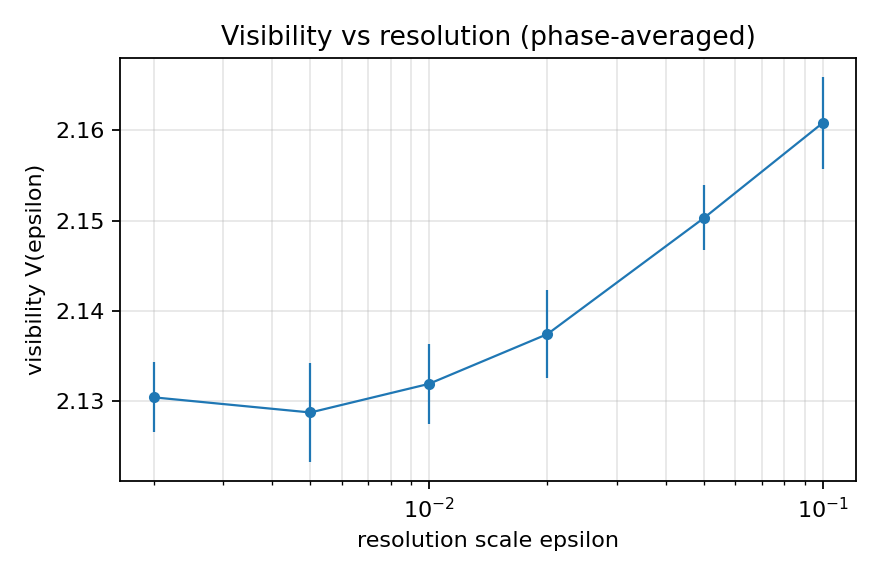
\includegraphics[width=0.75\linewidth]{sections/generated/demo_2d_visibility_curve.png}
  \caption{Demo B: phase-averaged visibility curve $V(\epsilon)$ under a fuzzified window with boundary layer scale $\epsilon$ (error bars: standard deviation over phases). Here $V(\epsilon)$ is the coefficient of variation of a binned intensity along the projected coordinate (see \texttt{artifacts/demo\_2d\_fingerprints.json} for the exact definition).}
  \label{fig:demo2d-visibility}
\end{figure}

\begin{figure}[t]
  \centering
  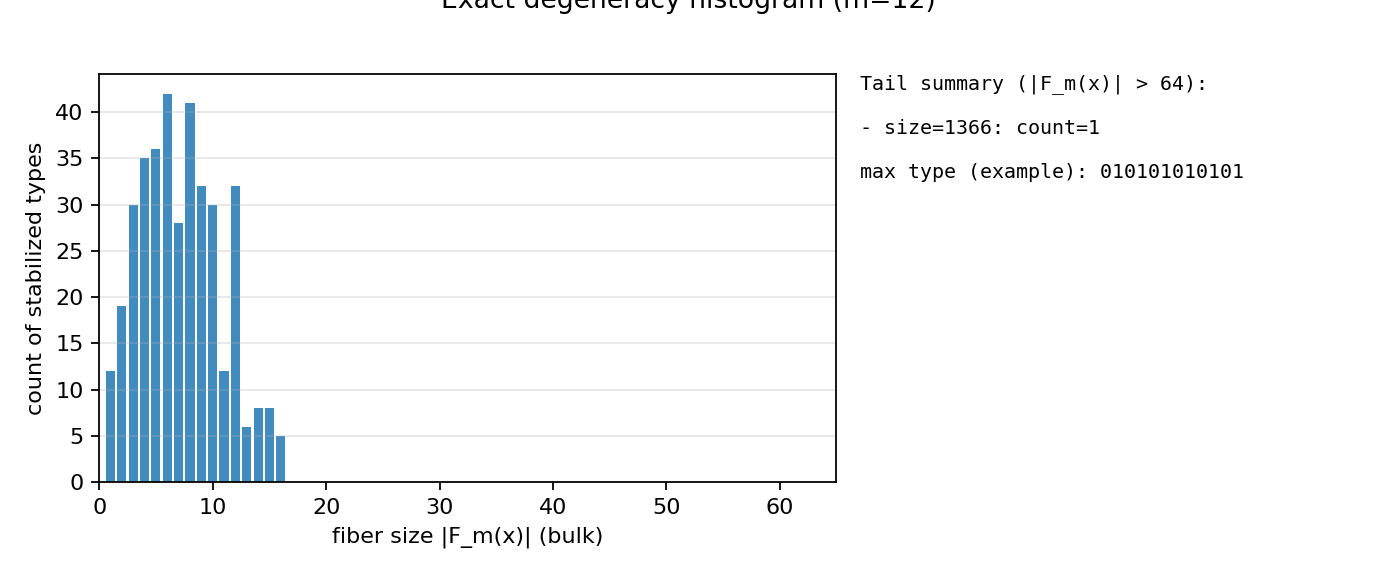
\includegraphics[width=0.9\linewidth]{sections/generated/demo_2d_degeneracy_hist.png}
  \caption{Demo B: an exact degeneracy histogram for a Zeckendorf-based $\Fold_m$ at fixed depth $m$. This provides a discrete, reproducible combinatorial invariant (cf.\ Proposition~\ref{prop:P3}) that can be compared to empirical stabilized-type statistics extracted from readout sequences.}
  \label{fig:demo2d-degeneracy}
\end{figure}

\begin{figure}[t]
  \centering
  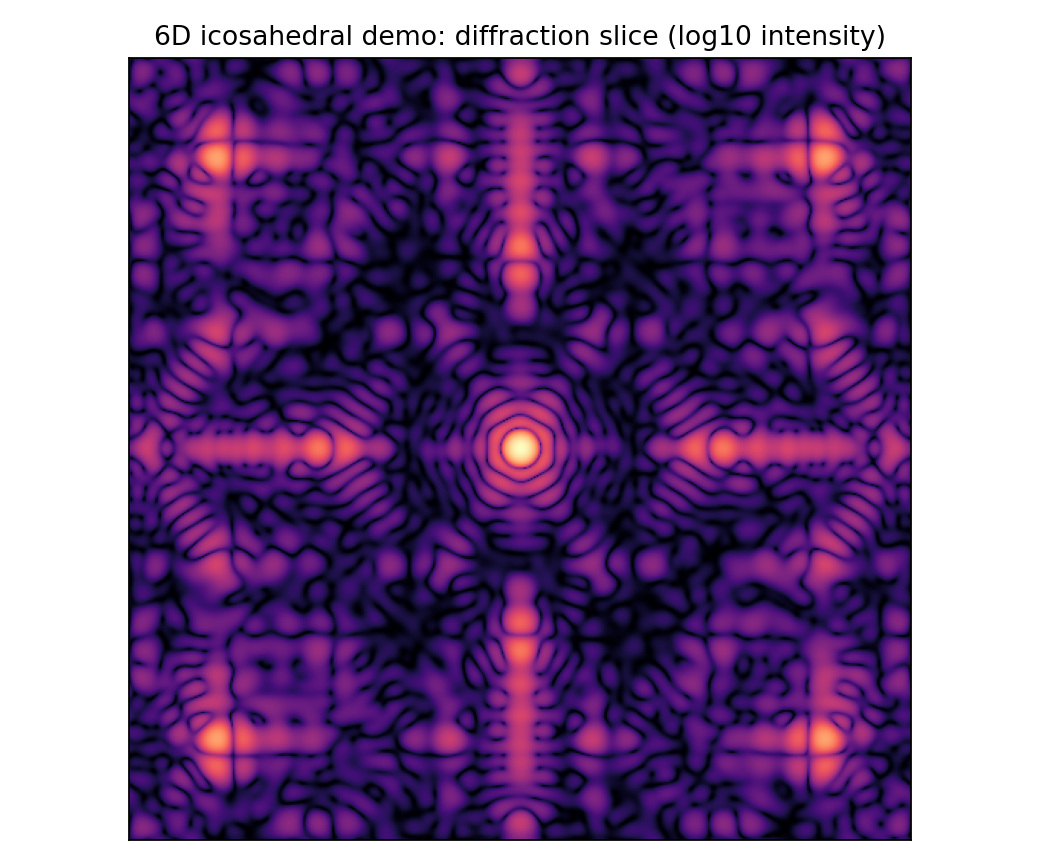
\includegraphics[width=0.75\linewidth]{sections/generated/demo_6d_diffraction_slice.png}
  \caption{Demo C: a 2D diffraction slice (log intensity) from a 6D $\ZZ^6$ cut-and-project construction using an icosahedral splitting (golden-ratio embedding) and a compact internal-space window. The slice is computed from an FFT of a binned projected density.}
  \label{fig:demo6d-diffraction}
\end{figure}

\begin{figure}[t]
  \centering
  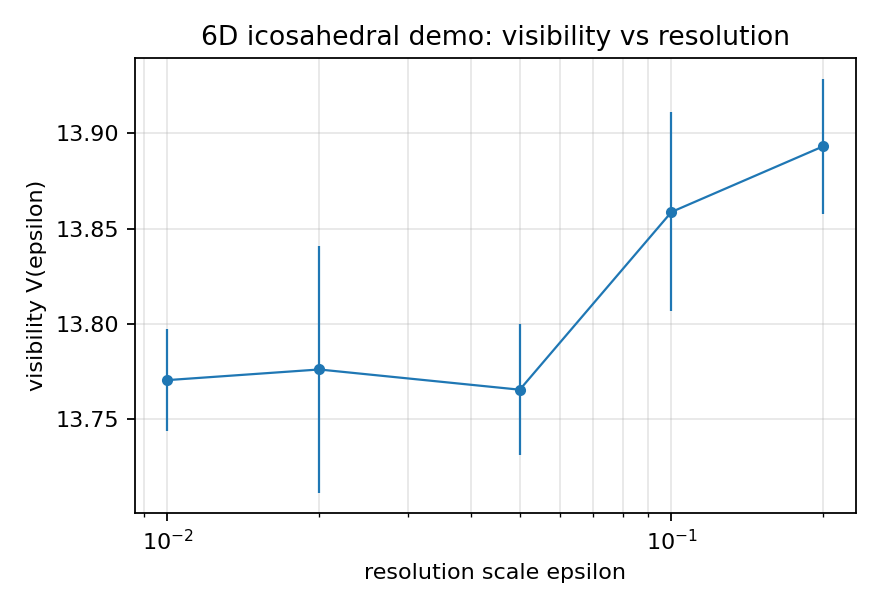
\includegraphics[width=0.75\linewidth]{sections/generated/demo_6d_visibility_curve.png}
  \caption{Demo C: phase-averaged visibility curve $V(\epsilon)$ for the 6D icosahedral approximation under a fuzzified internal-space window (error bars: standard deviation over phases). Here $V(\epsilon)$ is the coefficient of variation of the binned projected density image used in the FFT slice.}
  \label{fig:demo6d-visibility}
\end{figure}

\begin{figure}[t]
  \centering
  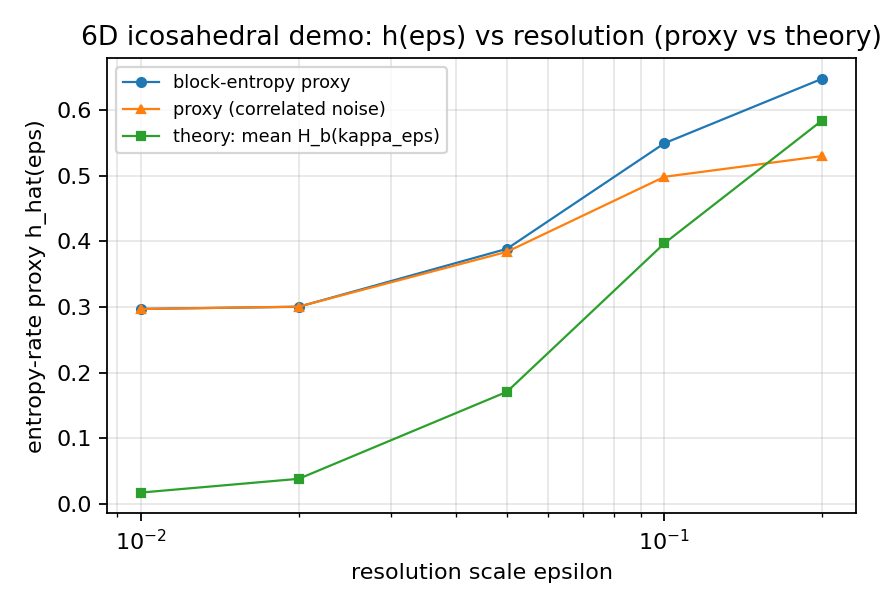
\includegraphics[width=0.75\linewidth]{sections/generated/demo_6d_entropy_rate_proxy.png}
  \caption{Demo C (symbolic scan): an entropy-rate proxy $\widehat h(\epsilon)$ estimated from block entropies of the binary record generated by an internal-phase scan with a probabilistic window kernel $\kappa_\epsilon$. As $\epsilon$ varies, the kernel changes the effective randomness and yields a reproducible $\epsilon$-dependence of information acquisition speed (cf.\ Remark~\ref{rem:noise-positive-entropy} and Definition~\ref{def:entropy-time}).}
  \label{fig:demo6d-entropy-rate}
\end{figure}

\begin{figure}[t]
  \centering
  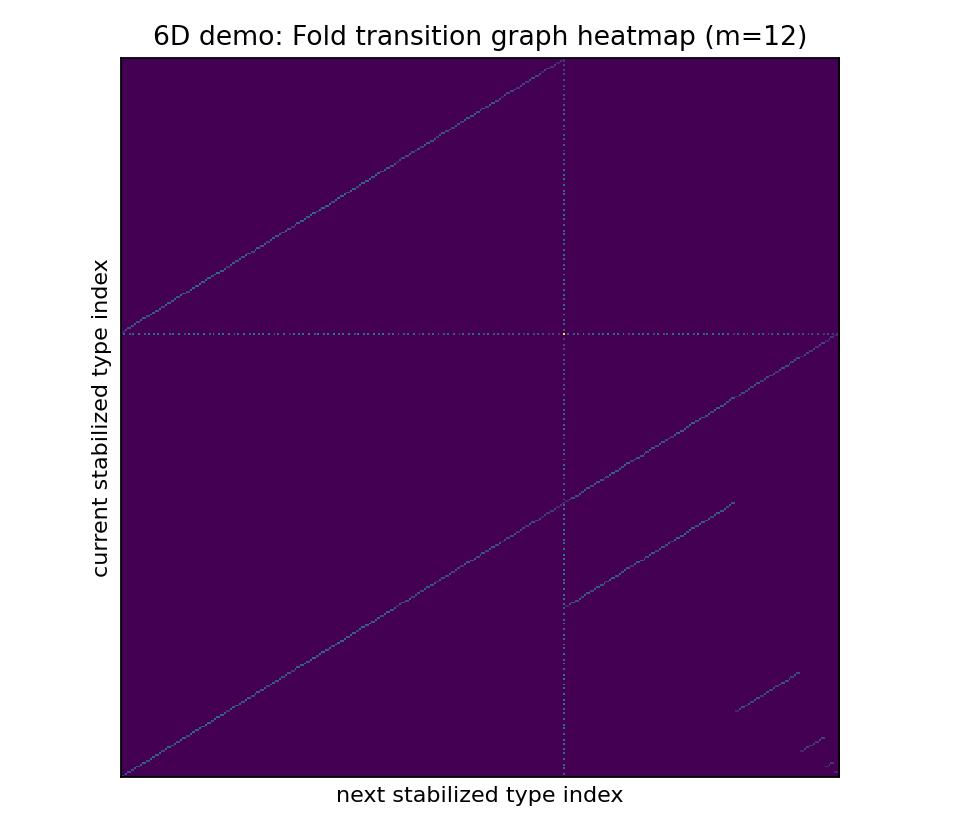
\includegraphics[width=0.75\linewidth]{sections/generated/demo_6d_fold_graph_m12_heatmap.png}
  \caption{Demo C (Fold transition graph): a heatmap visualization (log edge counts) of the exact stabilized-type transition graph induced by the Zeckendorf $\Fold_m$ at the reference depth $m=12$. Nodes are stabilized types; edges correspond to one-step shifts of raw length-$(m+1)$ words followed by stabilization.}
  \label{fig:demo6d-fold-graph}
\end{figure}

\begin{figure}[t]
  \centering
  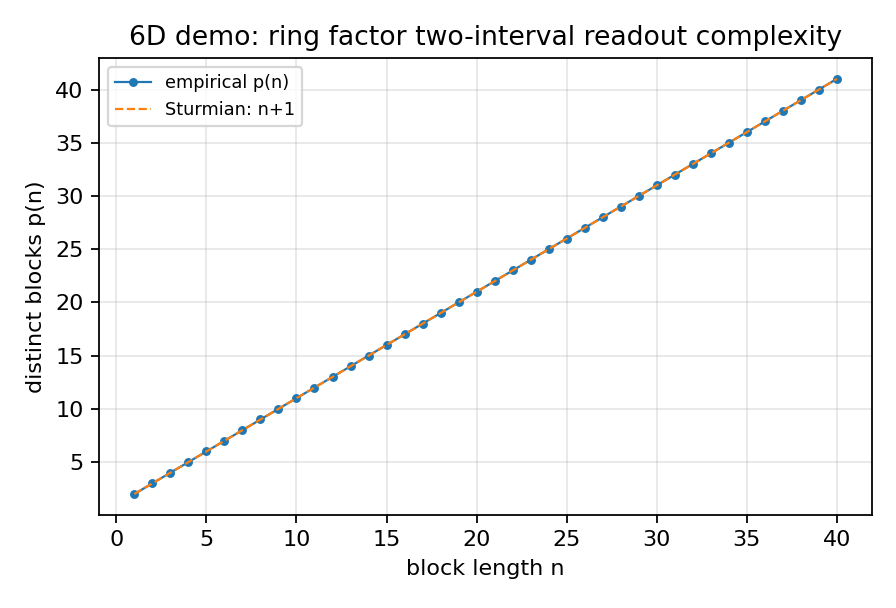
\includegraphics[width=0.75\linewidth]{sections/generated/demo_6d_ring_factor_complexity.png}
  \caption{Demo C (ring-factor cross-check): block complexity $p(n)$ for a two-interval readout of an irrational circle rotation (Sturmian regime). For irrational slope and a nondegenerate two-interval partition, one expects $p(n)=n+1$.}
  \label{fig:demo6d-ring-complexity}
\end{figure}

\begin{figure}[t]
  \centering
  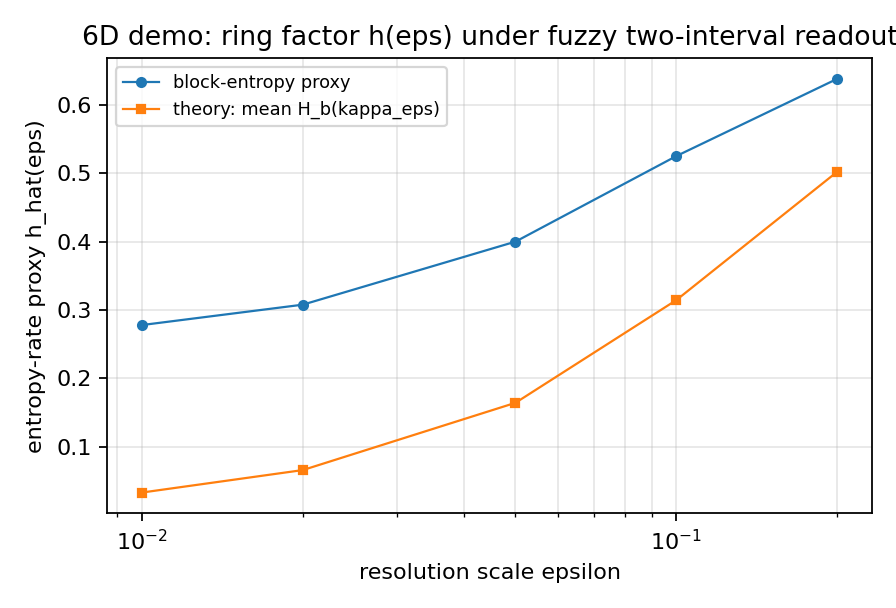
\includegraphics[width=0.75\linewidth]{sections/generated/demo_6d_ring_entropy_rate_proxy.png}
  \caption{Demo C (ring-factor cross-check): kernel-induced entropy-rate under a fuzzy two-interval readout on a deterministic rotation base. The plot shows a finite-data proxy $\widehat h(\epsilon)$ (block entropy at fixed block length) together with a theoretical comparator $\mathbb{E}[H_b(\kappa_\epsilon(x_t))]$ for the Bernoulli layer.}
  \label{fig:demo6d-ring-entropy}
\end{figure}

\subsection{Practical data strategy: finite-size effects and phase averaging}\label{sec:falsifiability:practice}

Empirical tests of quasi-periodic and entropy-rate claims are sensitive to finite-size effects. A practical strategy is therefore to treat \emph{phase averaging} and \emph{scaling checks} as mandatory rather than optional:
\begin{itemize}[leftmargin=*,itemsep=2pt]
  \item \textbf{Phase sampling}: repeat simulations (or experiments) for multiple internal phases $u$ and quantify phase-to-phase variance. For uniquely ergodic regimes, this variance should decay with sample size and reveal structured phase shifts rather than random drift.
  \item \textbf{Window/resolution scaling}: vary window width $\epsilon$ and word length $m$ in controlled grids; distinguish monotone trends from quasi-periodic modulation by fitting across scales rather than at a single scale.
  \item \textbf{Null-model controls}: compare against randomized phase shuffles or against rational approximants $\alpha_k=p_k/q_k$ to separate periodic-locking artifacts from genuinely quasi-periodic signatures.
  \item \textbf{Error budgeting}: report uncertainties from finite patch size, finite scan length $T$, and finite discretization of windows/kernels; where possible, use bootstrap estimates on symbolic blocks to quantify entropy-rate estimator error.
\end{itemize}

These steps are essential if the results are to be persuasive to GRG reviewers: the core claims live at the level of invariant statistics, and invariants only become visible through careful control of finite-sample distortions.

\begin{remark}[Quantifying protocol-variation error bars]\label{rem:protocol-variation-errorbars}
When comparing two nearby protocols (e.g.\ window width $\epsilon$ vs.\ $\epsilon'$, or two partitions/codings, or a noisy vs.\ noiseless readout), one can estimate the empirical one-step mismatch rate $\widehat\varepsilon$ by running the protocols on matched phases/trajectories and measuring the Hamming disagreement rate. Proposition~\ref{prop:entropy-continuity-mismatch} then yields an explicit per-symbol bound on the induced entropy-rate variation, while Proposition~\ref{prop:block-tv-by-mismatch} provides a finite-$t$ block-law control useful for error budgets of block-entropy estimators.
\end{remark}

\subsubsection{Finite-sample error bars and sample complexity (detectability thresholds)}\label{sec:falsifiability:sample-complexity}

The fingerprints in Propositions~\ref{prop:P1}--\ref{prop:P3} are asymptotic/invariant statements. To make them falsifiable in finite data, one needs explicit error bars and a minimal sample-length criterion.

\begin{proposition}[Mismatch-rate confidence bounds from a finite record]\label{prop:mismatch-hoeffding}
Let $(A_t,B_t)$ be a coupled pair of symbol streams on a finite alphabet, and let
\[
\widehat\varepsilon_N:=\frac{1}{N}\sum_{t=0}^{N-1}\mathbf{1}\{A_t\neq B_t\}
\]
be the empirical mismatch rate from a length-$N$ record. If $(\mathbf{1}\{A_t\neq B_t\})$ are independent Bernoulli trials with mean $\varepsilon$, then for every $\delta\in(0,1)$,
\[
\mathbb{P}\bigl(|\widehat\varepsilon_N-\varepsilon|\ge u\bigr)\ \le\ 2e^{-2Nu^2},
\qquad
u=\sqrt{\frac{\log(2/\delta)}{2N}}.
\]
Equivalently, with probability at least $1-\delta$ one has $|\widehat\varepsilon_N-\varepsilon|\le \sqrt{\tfrac{\log(2/\delta)}{2N}}$.
\cite{Hoeffding1963}
\end{proposition}

\begin{remark}[Correlated noise: effective sample size]
If the mismatch indicators are correlated (e.g.\ because the auxiliary noise source has correlation time), the same bound does not apply verbatim; in practice one replaces $N$ by an \emph{effective} sample size $N_{\mathrm{eff}}$ determined by the correlation length (block bootstrap provides an auditable estimate). This is the same phenomenon as in Remark~\ref{rem:correlated-diagnostics}: correlations inflate uncertainty bands and increase required record lengths.
\end{remark}

\begin{proposition}[A deterministic slope-separation scale for two-interval rotation codings]\label{prop:slope-separation-hamming}
Consider two circle rotations with slopes $\alpha,\alpha'\in(0,1)$ and a two-interval coding $R$ with boundary point $b\in\TT$ (the Sturmian/mechanical setting of Section~\ref{sec:readout:sturmian}). Let $a^{(\alpha)}_{0:N-1}$ and $a^{(\alpha')}_{0:N-1}$ be the resulting length-$N$ coded prefixes from the same initial phase. Then the Hamming mismatch count satisfies the deterministic bound
\[
\#\{0\le t<N:\ a^{(\alpha)}_t\neq a^{(\alpha')}_t\}\ \le\ 2N|\alpha-\alpha'|+2,
\]
hence the mismatch rate is $O(|\alpha-\alpha'|)$ at fixed $N$.
\end{proposition}

\begin{remark}[Rule-of-thumb for minimal data length to distinguish nearby slopes]
To statistically separate a ``golden-branch'' slope $\alpha$ from a nearby slope $\alpha'$ using a mismatch-based test, one needs a record long enough that the induced mismatch signal exceeds both (i) finite-sample uncertainty and (ii) observation noise.
A conservative, protocol-facing rule-of-thumb is:
\[
N \gtrsim \max\Bigl\{\frac{1}{|\alpha-\alpha'|},\ \frac{\log(1/\delta)}{(\Delta\varepsilon)^2}\Bigr\},
\qquad \Delta\varepsilon\asymp c\,|\alpha-\alpha'|,
\]
where $\Delta\varepsilon$ is the expected mismatch-rate gap under the chosen coupling and $\delta$ is the target false-alarm probability. The first term enforces that the two rotations drift by an $O(1)$ phase over the record (otherwise the codings can coincide on a long prefix), while the second term is the usual $1/(\text{signal})^2$ sampling cost of estimating a Bernoulli rate.
In practice, a sharper and more falsifiable strategy is to compare $\alpha$ against its continued-fraction convergents $p_k/q_k$ as null models (finite-prefix periodic lock-in) and to report the deviation metrics (periodicity error at $q_k$, three-gap statistics, and Hamming mismatch) with bootstrap confidence bands (Demo~C archives these quantities in \texttt{artifacts/demo\_6d\_fingerprints.json}).
\end{remark}

\subsection{A reproducibility checklist}\label{sec:falsifiability:repro}

Because the claims in this review are primarily about invariant statistics and protocol-defined quantities, a minimal reproducibility checklist is particularly straightforward:
\begin{itemize}[leftmargin=*,itemsep=2pt]
  \item Record the full protocol specification $\Theta$ (window family, resolution kernel, scan rule, stabilization rule $\Fold_m$, and all truncation conventions).
  \item Fix random seeds whenever probabilistic readout is used (e.g.\ kernel-induced Bernoulli sampling) and report them.
  \item Report the phase-sampling scheme (how $u$ or $h_0$ are chosen) and the number of phases used.
  \item Provide the finite-size schedule (patch sizes, scan length $T$, and the range of $(m,\epsilon)$ tested) and show convergence trends rather than single-scale snapshots.
  \item Archive raw outputs and post-processed statistics (diffraction estimates, entropy estimates, degeneracy histograms) in a form that allows independent recomputation.
\end{itemize}
Meeting these conditions is often sufficient to make disagreements about interpretation secondary: independent groups can at least verify whether the same geometry+protocol chain reproduces the same fingerprints.

In particular, for review-style contributions such as the present one, reproducibility is best served by making the protocol explicit enough that a reader can implement it independently from scratch, without relying on undocumented conventions. This is also the most direct route to meaningful falsifiability: if the protocol cannot be reproduced, neither can the claimed invariants.

